\section{Time box 2}
\subsection{Time box planning}
Overview of the what work is put into which time boxes.
\begin{figure}[H]
	\begin{centering}
		 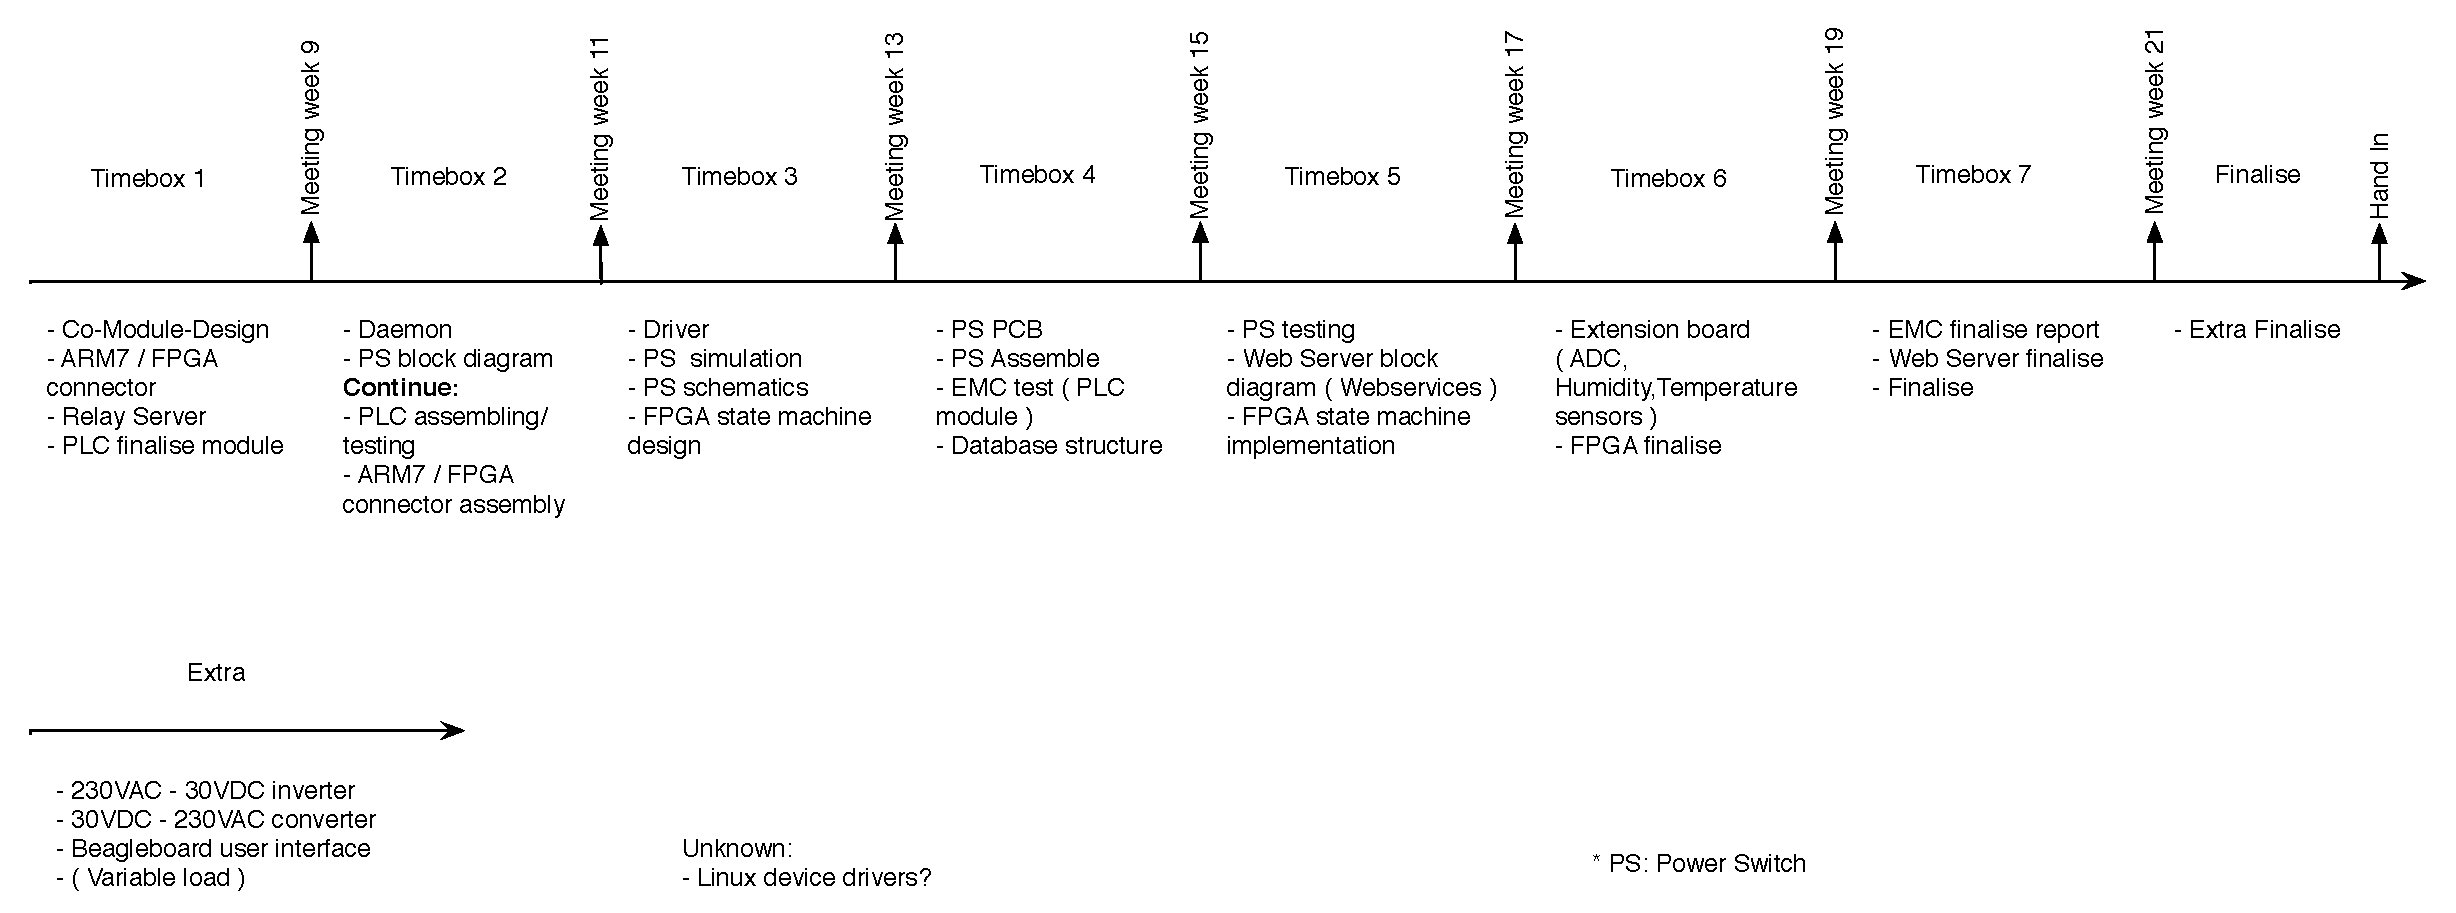
\includegraphics[width=1.0\textwidth]{images/tb_r2.pdf}
		\caption{Updated time-box}
	\end{centering}
\end{figure}

\subsubsection{Work to be done in this time box}
\begin{itemize}
	\item ARM7 to Spartan6 interface
	\begin{itemize}
		\item Mount
		\item Test
	\end{itemize}
	\item PLC module
	\begin{itemize}
		\item Mount x6
		\item Test
	\end{itemize}
	\item Daemon
	\begin{itemize}
		\item Overview
		\item Background process on uClinux
		\item The rc file (startup file)
		\begin{itemize}
			\item Configure network
			\item Start daemon as background process
		\end{itemize}
		\item Further implementations
		\item Documentation
	\end{itemize}
	\item Power switch
	\begin{itemize}
		\item Block diagram
	\end{itemize}
	\item Module design
\end{itemize}
\paragraph{Description:}
\begin{description}
	\item[ARM to Spartan6 interface] The interface between the ARM7 CPU and the Spartan6 board, has to be mounted and tested. 
	\item[PLC module] The powerline module has to be mounted 6 times, in order to provide one for all the groups. The boards should also be tested and debugged.
	\item[Daemon]  Create a program that runs as background process, there is no direct control between user and the application.
	\item[Power switch] Block diagram of the power switch, which shall activate the different modules connected to it (wind-turbine, photo-voltaic cells etc.) and control the current flow.
	\item[Module design] is an overview of the part connection in the system
\end{description}

\subsection{ARM to Spartan6 interface - Dennis}
The first version of the PCB was hard to solder because of the small pad sizes. A second version of the interface has been made, with increased pad size and increased clearance between the tracks. Also the Chip select connector pin has been more centralized on the PCB to decrease cable length. The hole in the one site of the PCB is needed to avoid removing a connector on the arm-board, the tracks beside this connector have been rerouted to give more space for this connector. 
\begin{figure}[H]
	\begin{centering}
		 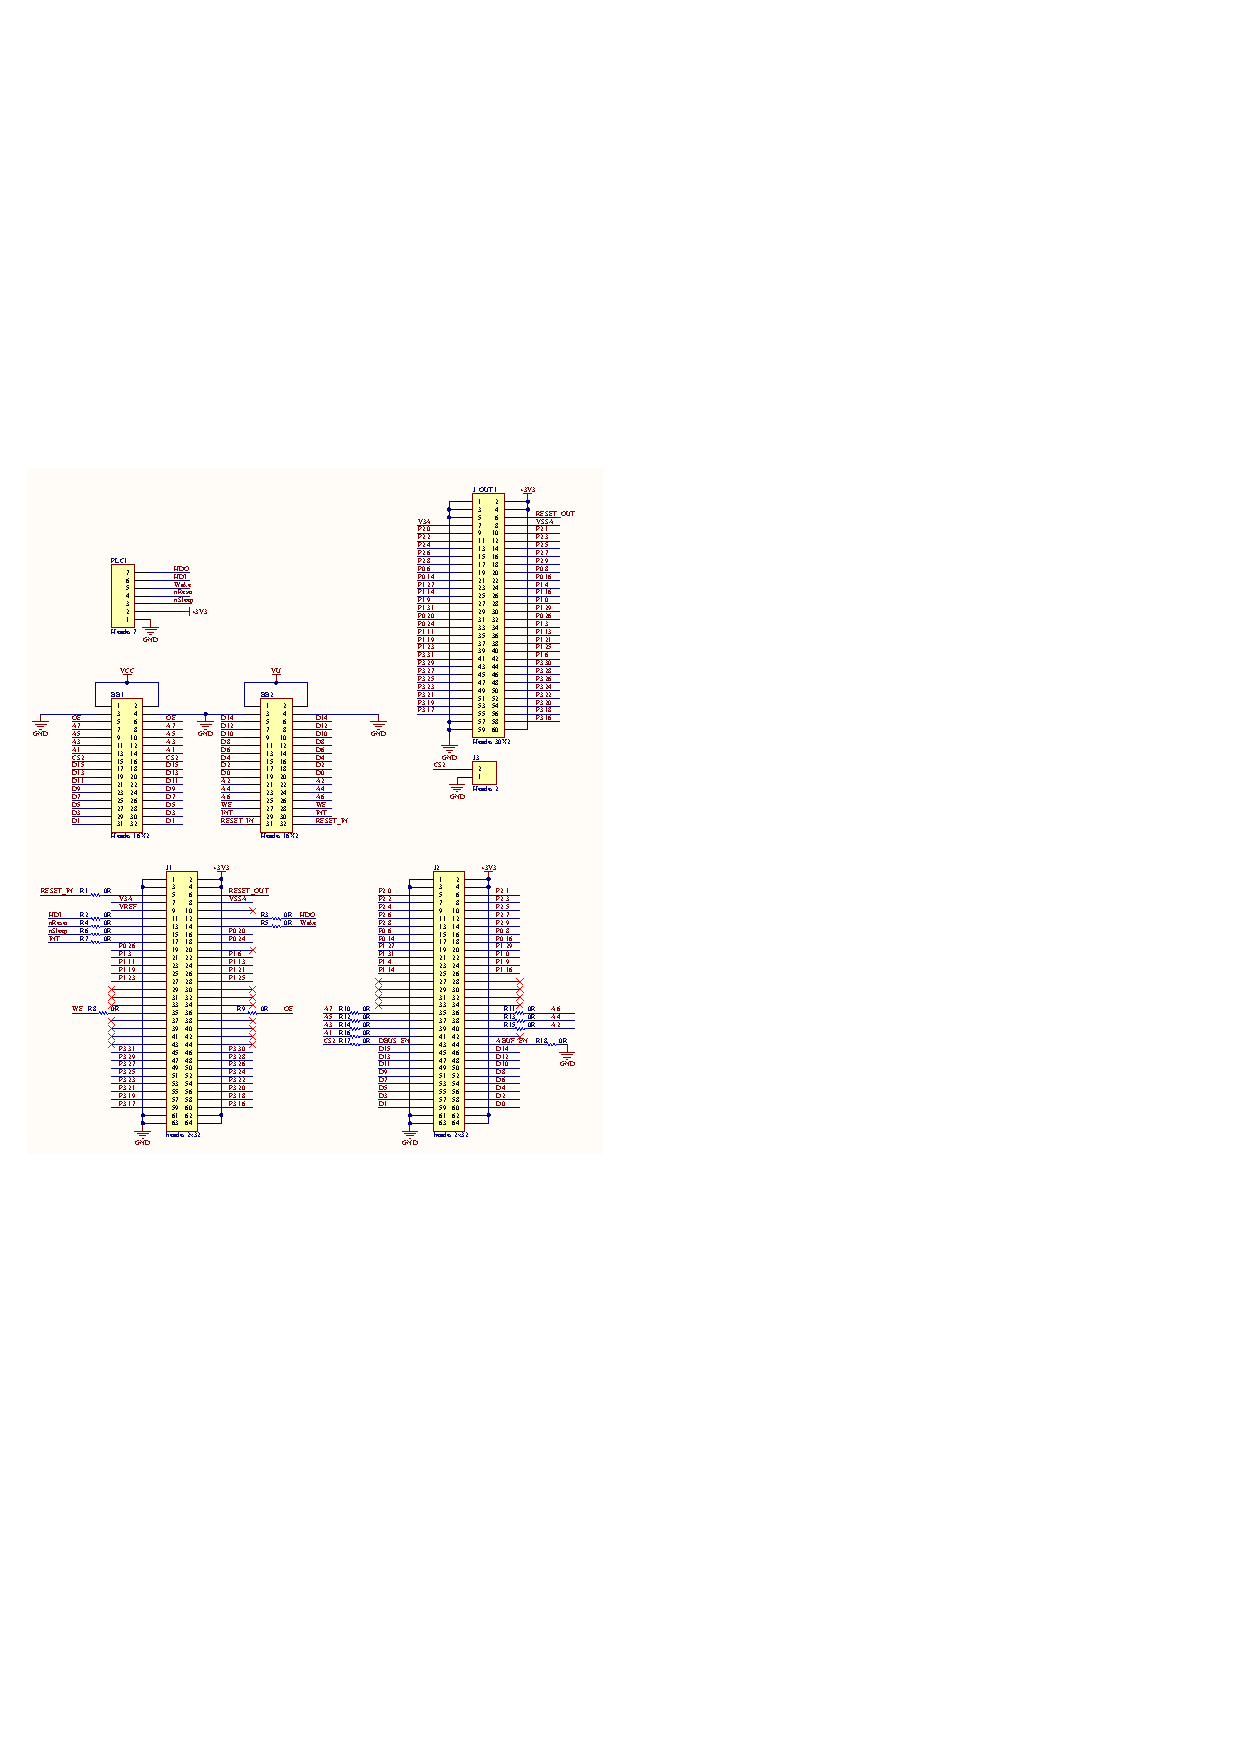
\includegraphics[width=0.60\textwidth,page=1]{images/dig_to_ea_v0_2}
		\caption{Schematic of the ARM to Spartan6 connector, v0.2.}
	\end{centering}
\end{figure}

\begin{figure}[H]
	\begin{centering}
		 \includegraphics[height=0.8\textwidth,page=2,angle=90]{images/dig_to_ea_v0_2}
		\caption{PCB of the ARM to Spartan6 connector, v0.2 (top view)}
	\end{centering}
\end{figure}

\begin{figure}[H]
	\begin{centering}
		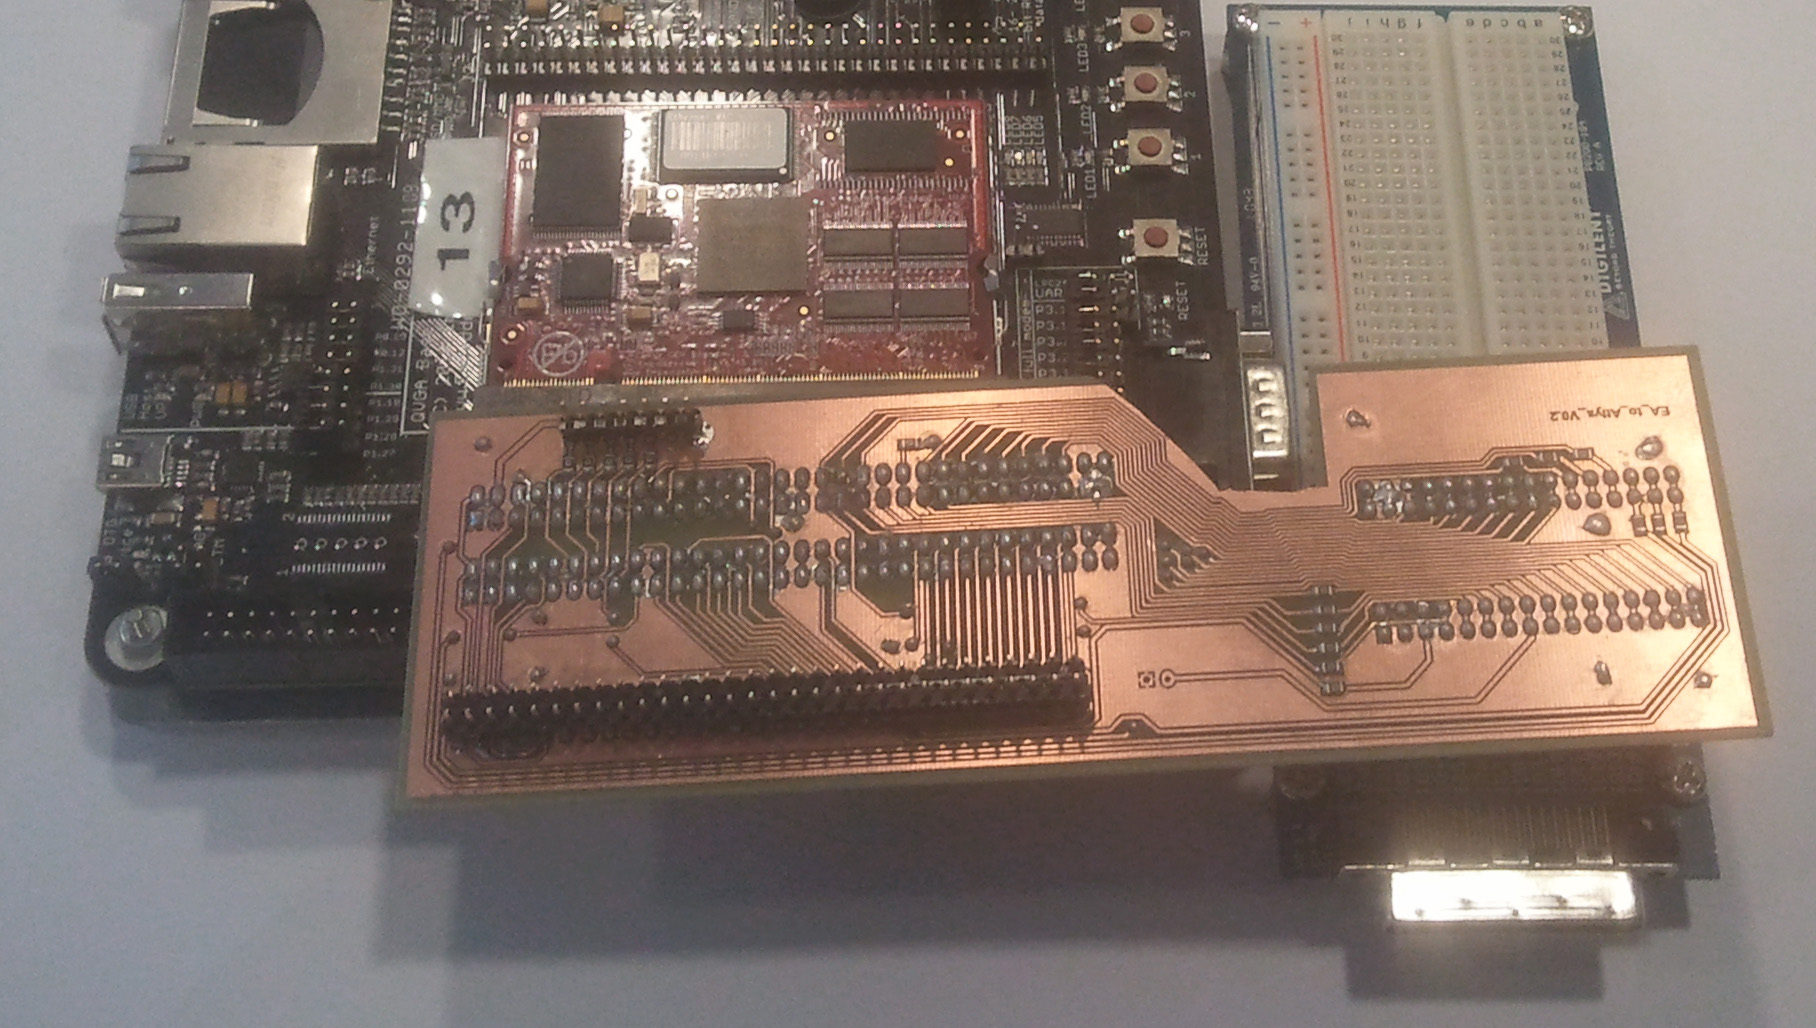
\includegraphics[width=0.8\textwidth,page=1,angle=0]{images/interface_photo_v0_2.jpg}
		\caption{Picture of the mounted interface PCB. The connector in the bottom right of the picture is the connection to the Diligent Spartan6 board.}
		\label{fig:interface_photo_v0_2}
	\end{centering}
\end{figure}

\subsection{PLC module - Dennis}
The second version of the Power line module was decreased in size, which lead to problems when making the PCB, as a lot of tracks short-circuited. A third version with larger clearance between the tracks and the ground plane has been made. The PCB has been mounted and tested, this is describe in the \textit{EPRO 3 \& 4 PLC - Hardware Interface} report. As a short resume, the communication between two boards through power line works without seeing any invalid characters (test period of 15 min.). The 5 volt power supply has been tester to withstand at minimum 2.4 Amp. where a voltage drop of approximately 0.1Volt was observed. 
A single error has been found and corrected before ordering and mounting the 6 PLC boards needed (one for each module in the system/group).

\begin{figure}[H]
	\begin{centering}
		 \includegraphics[width=0.9\textwidth,page=2,angle=0]{images/SIG60_v0_4}
		\caption{Power line circuit version 0.4}
	\end{centering}
\end{figure}

\begin{figure}[H]
	\begin{centering}
		 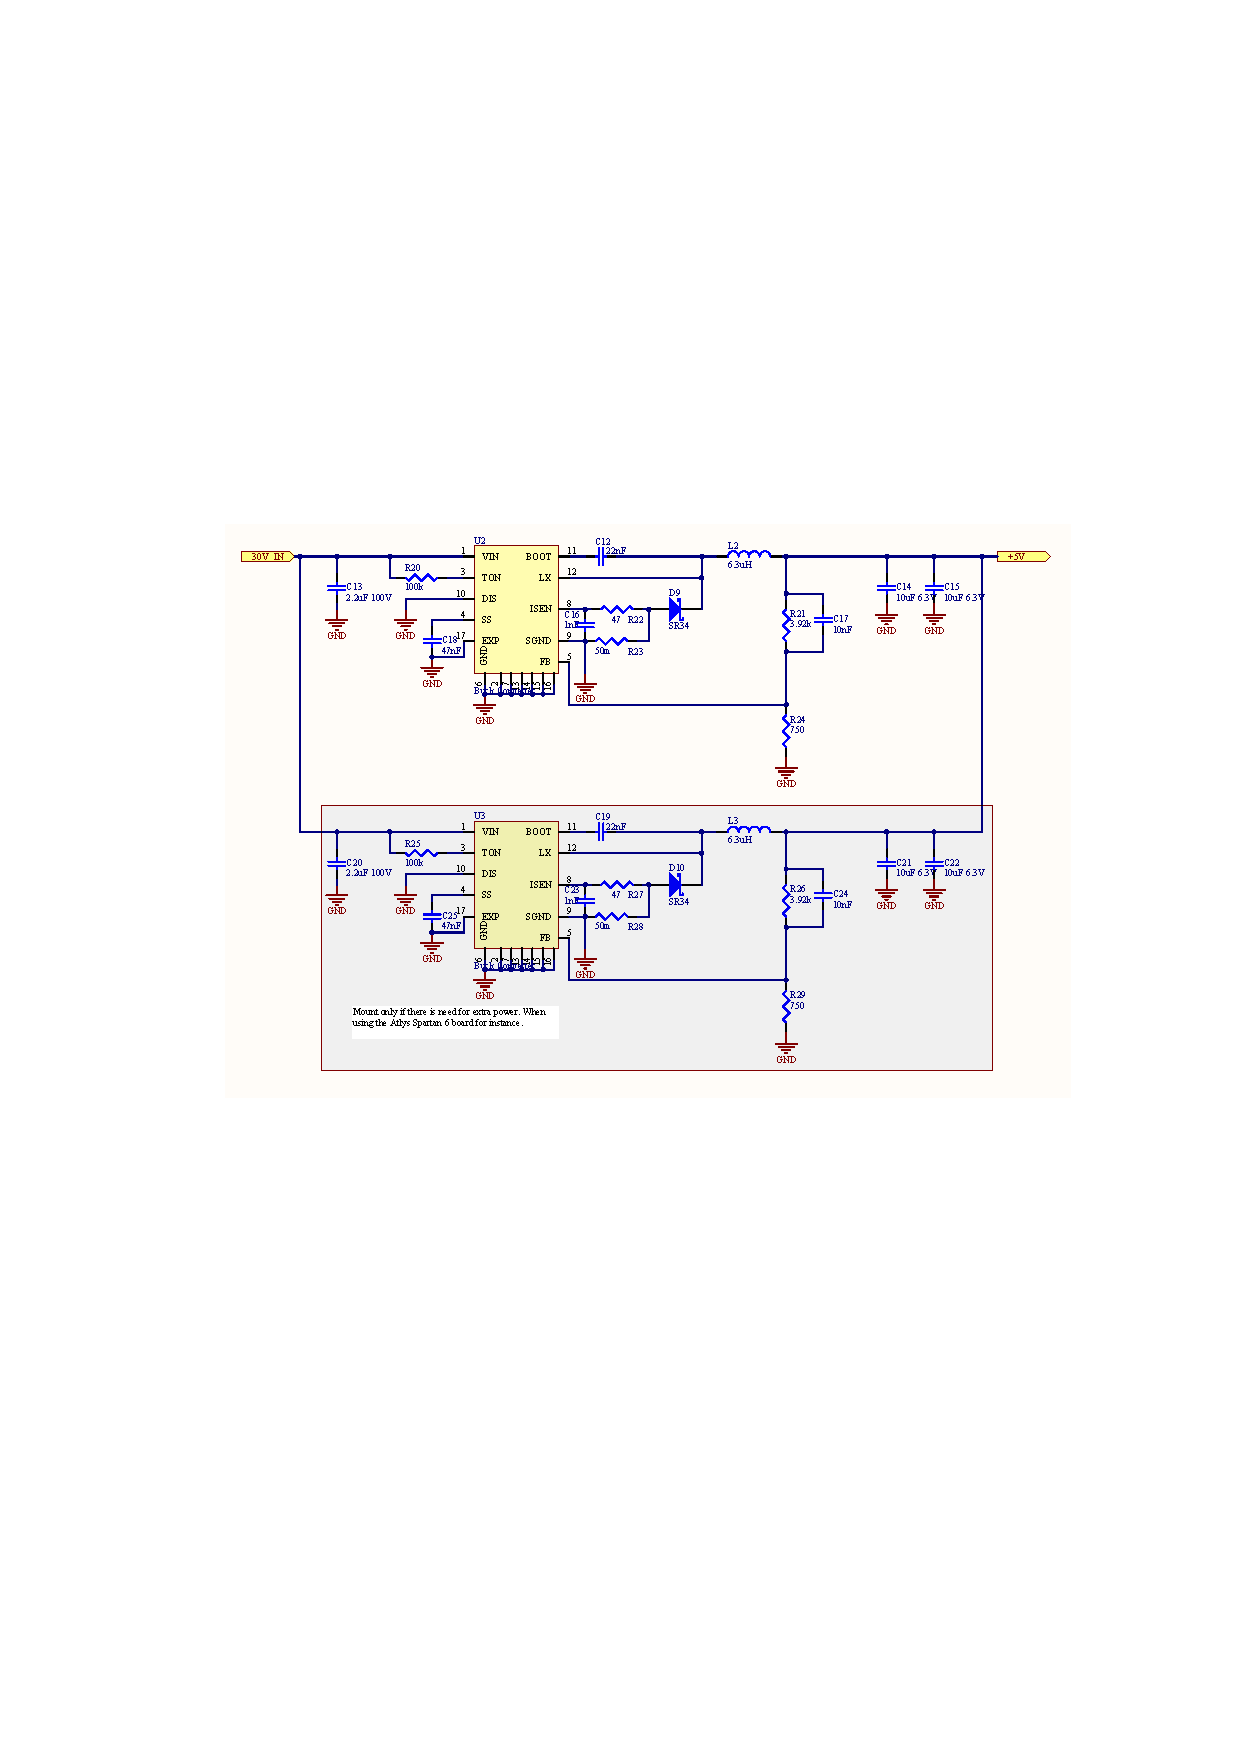
\includegraphics[width=0.8\textwidth,page=1,angle=0]{images/SIG60_v0_4}
		\caption{Power supply. 2 x 5 volt 3 ampere version 0.4.}
	\end{centering}
\end{figure}

\begin{figure}[H]
	\begin{centering}
		 \includegraphics[width=0.7\textwidth,page=3,angle=0]{images/SIG60_v0_4}
		\caption{PCB layout of the power line circuit and the 5 volt power supply version 0.4.}
	\end{centering}
\end{figure}

\begin{figure}[H]
	\begin{centering}
		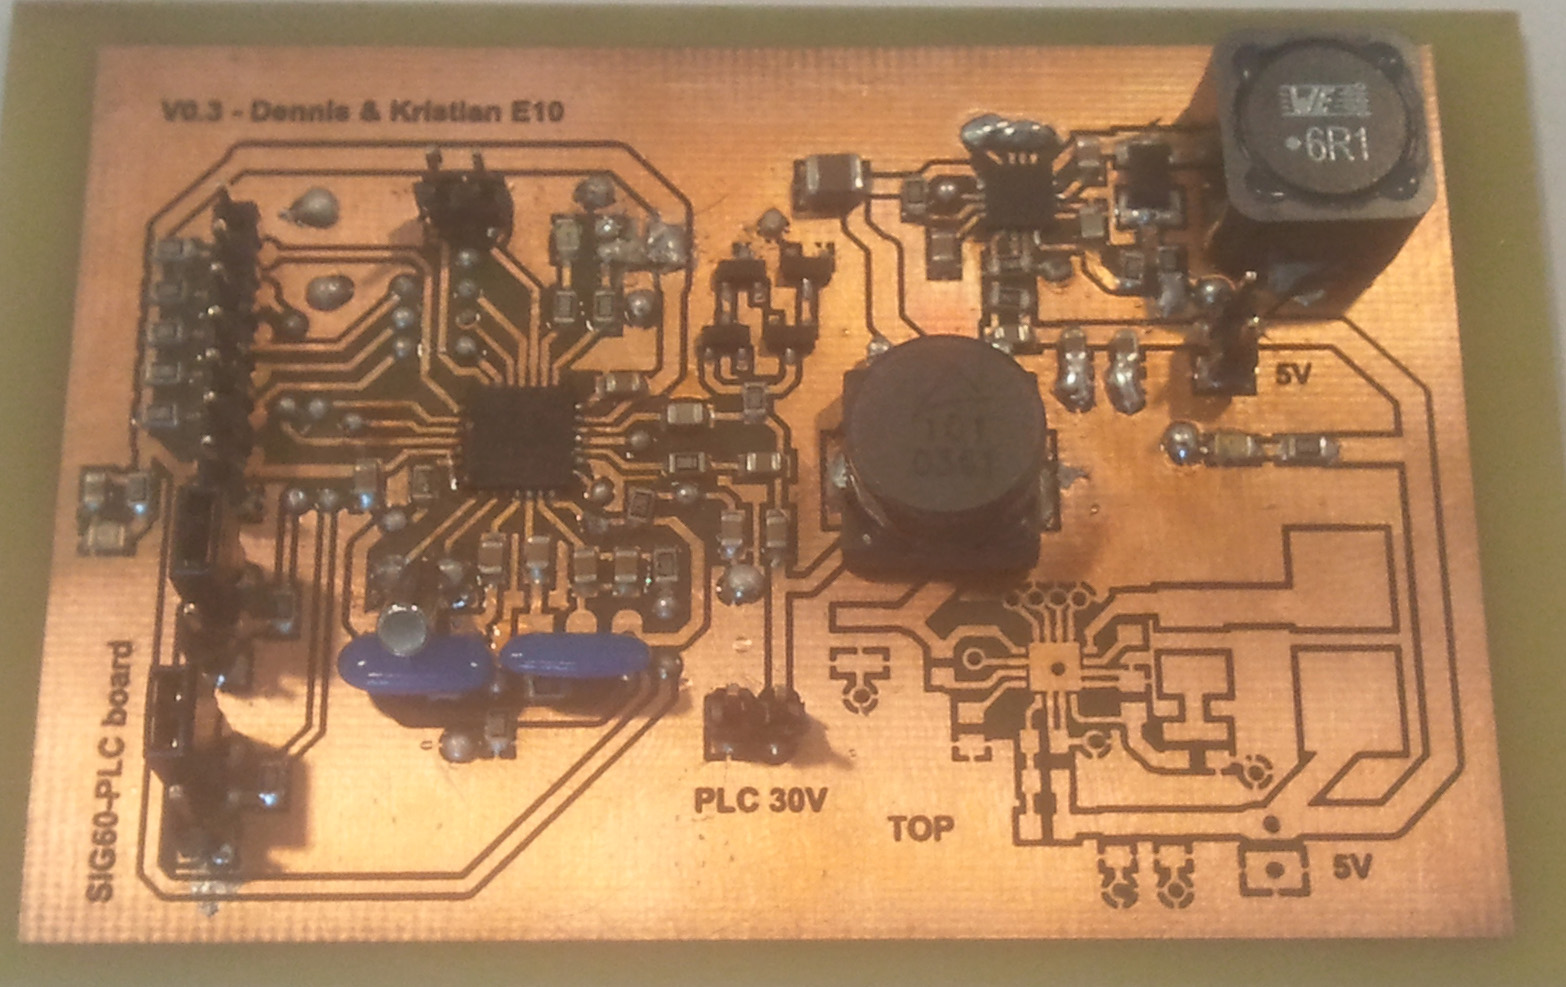
\includegraphics[width=0.6\textwidth,page=1,angle=0]{images/plc_photo_v0_3.jpg}
		\caption{Picture of the mounted PLC board (note, only one of the supplies is mounted)}
		\label{fig:plc_photo_v0_3}
	\end{centering}
\end{figure}

\subsection{Daemon}
\subsubsection{Section Contents}
\begin{itemize}
	\item Overview
	\item Background process on uClinux
	\item The rc file (startup file)
	\begin{itemize}
		\item Configure network
		\item Start daemon as background process
	\end{itemize}
	\item Further implementations
	\item Documentation
\end{itemize}

\subsubsection{Overview}
Daemon is a program that runs as background process, there is no direct control between user and the application.

The background application is going to establish a socket ( way of communication through network ), that will allow TCP connections to port 5555 of the LPC2478 Development board running the uClinux. This distribution can be found at \footnote{\url{http://uclinux.org/}}.

In further development of this application, the user is able to get status from the device by connecting to it using a TCP client (Putty, coolTerm, HyperTerminal, etc).

In this version the user is able to light all the four LEDs on the development board by typing the command: led \textless number of the led to light on\textgreater  \textless on/off\textgreater

\subsubsection{Background process on uClinux}
A background process is an application that is disassociated from the initial terminal. 

To make a application run as a process in UNIX environment:

\begin{itemize}
	\item Create a separate process.
	\item Detach the process from the parent.
	\item Reset file mask.
	\item Change the current directory.
	\item Close the standard files ( STDIN, STDOUT, STDERR ).
\end{itemize}

uClinux distribution runs on embedded system and since most of them don't have a MMU (memory management unit), the fork() function is not allowed int this implementation.

The fork() function when called causes the creation of a new process (child process). The child process will be a exact same copy of the parent process being this impossible without a MMU.
To implement the same functionality the vfork() function is use, this function creates a new process but the memory address is shared by the parent and child.

\subsubsection{The rc file (startup file)}
The rc is a file that contains the startup instructions for the operation system in use (uClinux) this file can be found at the specific vendor folder. 
This file contains commands that will run automatically each time the system starts.
\paragraph{Configure Network}
When the system starts the network have to be configured so the device can be part of our network. The configuration can be done manually each time with the commands:

ifconfig eth0 x.x.x.x netmask x.x.x.x up

route add default gw x.x.x.x

being x.x.x.x ip adresss.

\newline
\newline
Defining this commands in the rc file will make the network to be always accessible after a reboot is needed, for example is a update is implemented to the software. 

\paragraph{Start daemon as background process}
The daemon is defined in this script by the command: daemon \& , this way the application run as background when the operating system starts, allowing the communication between the device and the user.

\subsubsection{Further implementations}
\begin{itemize}
	\item A background application will be implemented to update data on a Mysql server and retrieve commands from the web server, this will be the pipe between all the modules in the system.
\end{itemize}


\subsubsection{Documentation}
This daemon (background application), is a TCP echo server, this means it will answer back the same message that was received. This was explain in Time box 1 along with the development of the relay server. 

In this TCP echo server, a command handler was implemented, this allow the user to turn on and off the LEDs on the development board: \textbf{led \textless number of the led to light on\textgreater  \textless on/off\textgreater}

The daemon is calling the application already existent in the development board made by Embedded Artists as example.

\subsection{Power switch - Dennis}
The power switch is the part of the hub that traffics the energy from and to its connected modules, such as: wind-turbine, photovoltaics, hydrogen-cell, battery-storage, load modules and similar. Inspiration to the creation of the power switch has been found at: Powerhub Systems \footnote{\url{http://www.pwrhub.com/}} (routing system) and TORC \footnote{\url{http://www.torcrobotics.com/products/powerhub}} (implementation and control of the hub).
\subsubsection{Block diagram}
The switch is divided in 10 similar blocks (one for each module). Figure \ref{fig:ps_block_v0_1} shows two modules connected to the power line. The content inside the dotted line block is an abstract description of the power switch. For simplicity two diodes has been used, to control the routing direction.
\begin{figure}[H]
	\begin{centering}
		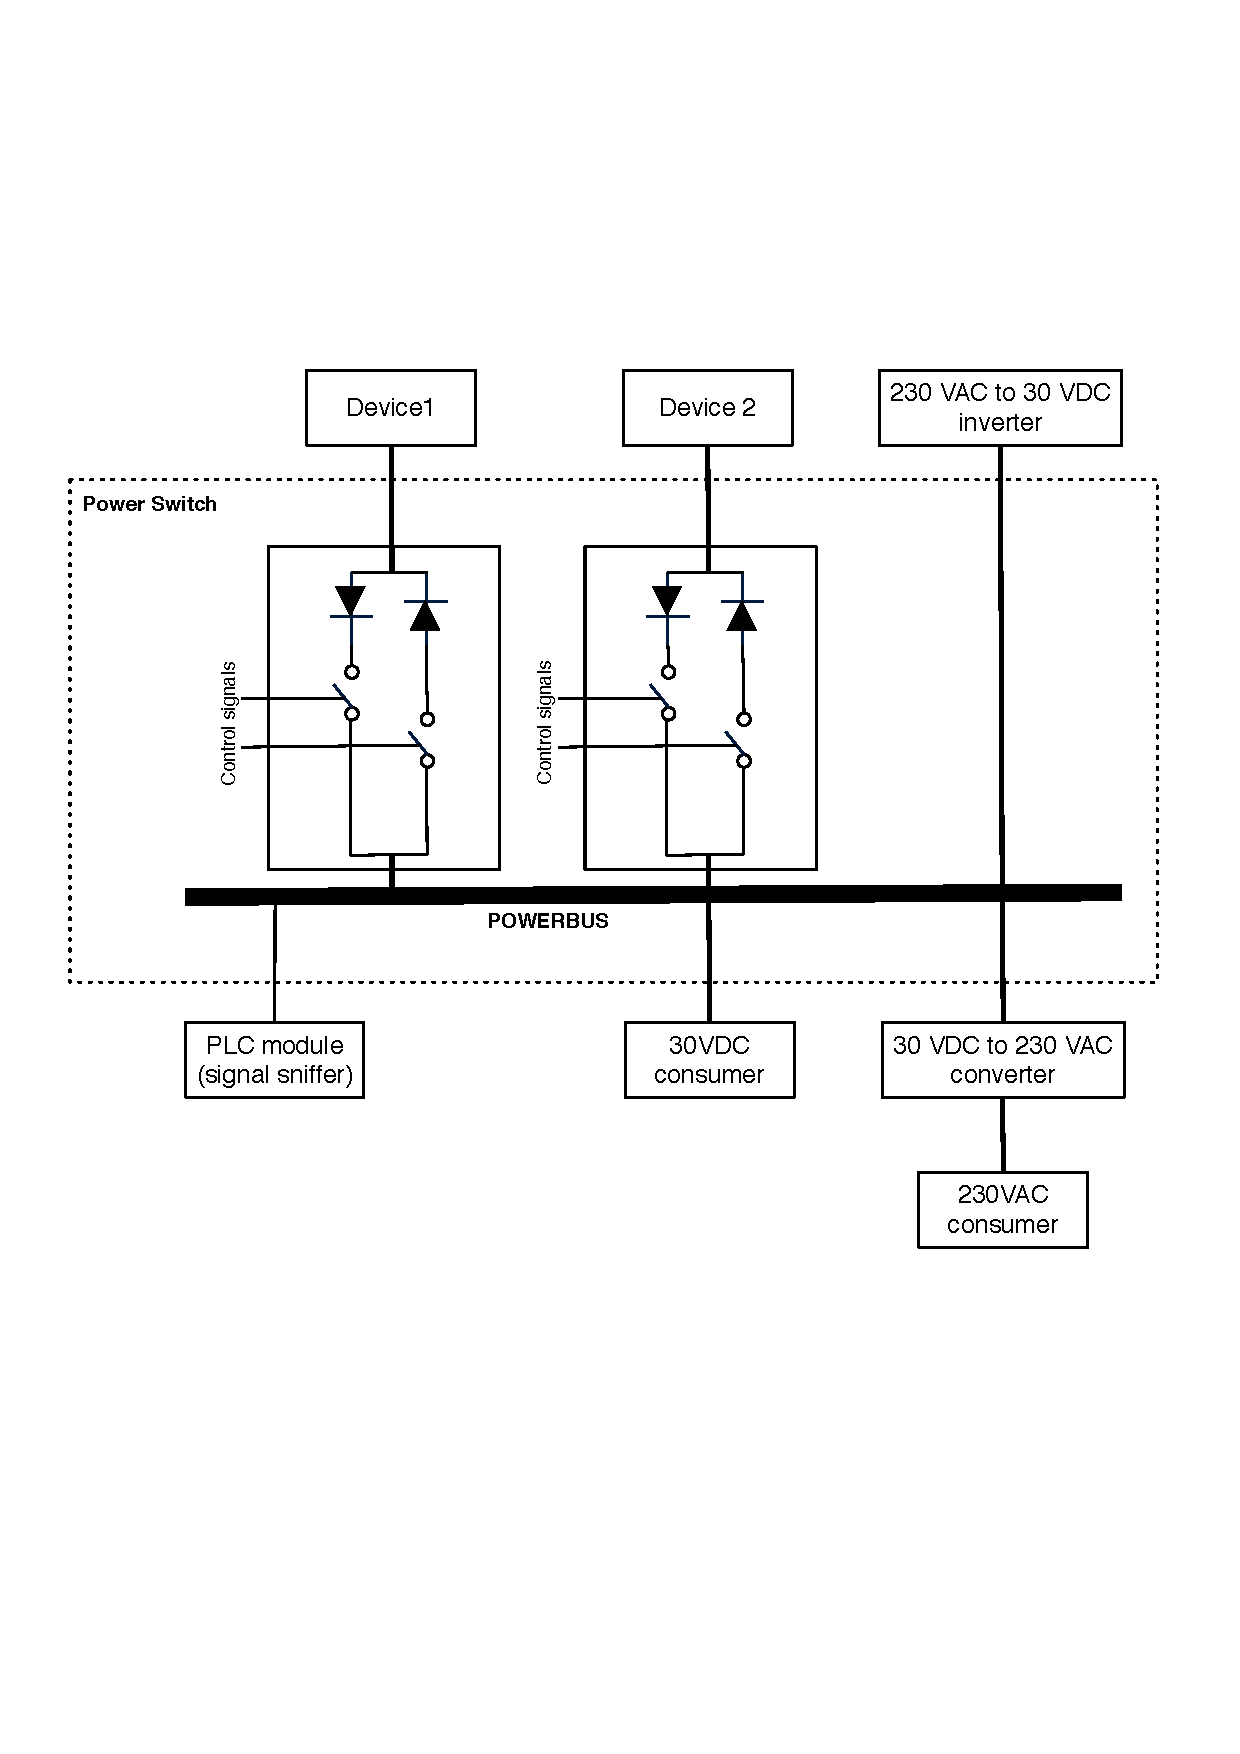
\includegraphics[width=0.8\textwidth,page=1,angle=0]{images/power_switch_block_diagram_v0_1}
		\caption{Block diagram of the Power Switch v0.1}
		\label{fig:ps_block_v0_1}
	\end{centering}
\end{figure}
The inverter is used to supply the system at startup time. The system is also supplied through the inverter if the energy-producing- and energy-storing modules cannot deliver enough energy. 
\p Notice that noise from switching devices on and off shall be minimized to not bother the power line module and in worst case manipulate with the data-packages. 
\p Two signals from the processor will be needed to control each of the switch blocks, however a control section might be added to the switch to decrease the number of pins needed to control all 10 blocks + consumers. 
\p Current measuring for the consuming devices and the inverter will be implemented in the switch, to keep track of how green the system is and if the producers are producing anything.  
\subsubsection{Diagram and components}
Some alternative components to diodes have been found, in order to control the current direction and have as little power loss as possible in the switch. 
\\\textbf{Component suggestions:}
\begin{itemize}
	\item Control device for MOSFETS, LTC4357\footnote{\url{http://www.linear.com/product/LTC4357}} from Linear Technology.
	\item Demo board for LTC4357\footnote{\url{http://cds.linear.com/docs/Demo\%20Board\%20Manual/dc1203A.pdf}}.
	\item Power Mosfets IRFP4468PbF\footnote{\url{http://pdf1.alldatasheet.com/datasheet-pdf/view/234175/IRF/IRFP4468PBF.html}} with low on resistance and maximum drain current of approximately 200Amps. \textit{Rds}
	\item If needed, an dual power rectifiers has been found: MBR60H100CT\footnote{\url{http://pdf1.alldatasheet.com/datasheet-pdf/view/172142/ONSEMI/MBR60H100CT.html}}, with max. voltage on 100V and max. current on 60 Amps.
\end{itemize}
An initial diagram drawing have been made with two LTC4357 devices. The diagram shows the possible implementation of a single switch block.

\begin{figure}[H]
	\begin{centering}
		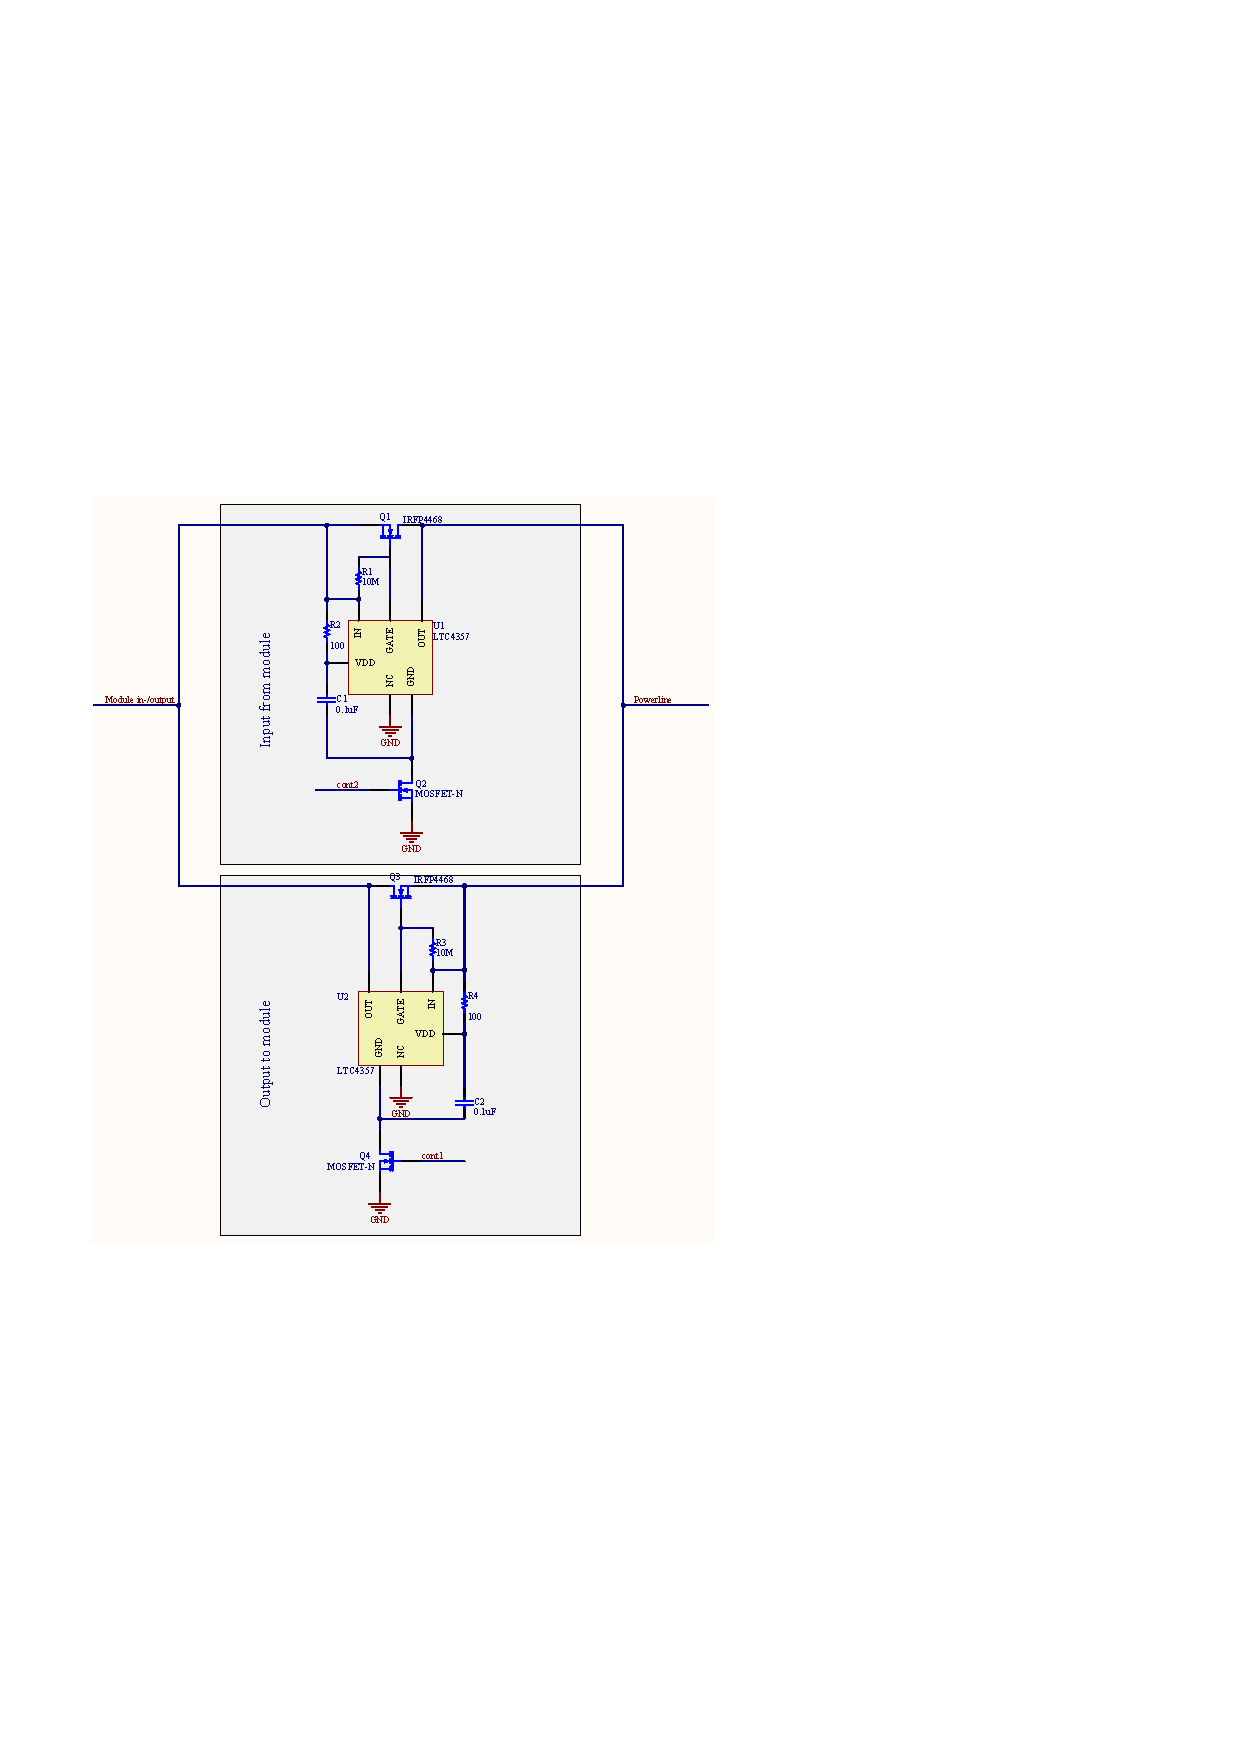
\includegraphics[width=0.75\textwidth,page=1,angle=0]{images/PS_initial_drawing.pdf}
		\caption{Power switch, diagram of a single switch block.}
		\label{fig:ps_switch_dia_v0_1}
	\end{centering}
\end{figure}
The system makes use of two LTC4357 to control the two MOSFETS used as diode substitutions. So far no protection circuit have not been added to the diagram, or multiplexing for the control signals, but only the basic concept of the switching mechanism.

\subsection{Module design}

The module design is to give an overview of the part connection in the system. On the module design is shown which parts shall be made in software and which parts shall be made in hardware. The connection between the parts is also shown, plus the connection to external parts.

\begin{figure}[H]
	\begin{centering}
		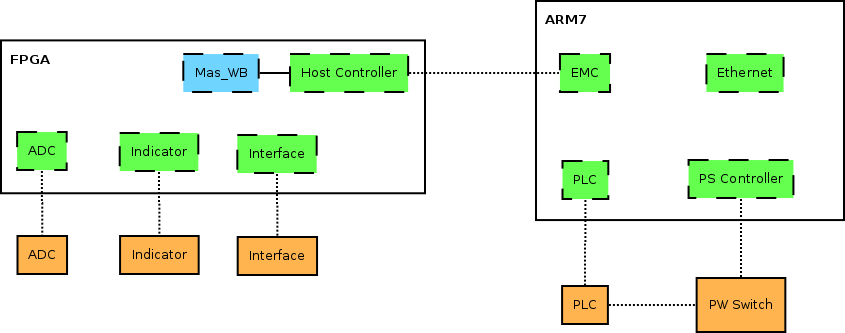
\includegraphics[width=0.8\textwidth,page=1,angle=0]{images/module_design.png}
		\caption{Module diagram}
		\label{fig:module_design_diagram}
	\end{centering}
\end{figure}

\textbf{Power line module}\\
In the table below the pin names on the PLC module and their corresponding pin on the ARM7 is listed.
\begin{table}[H]
    \begin{tabular}{|p{4cm}|p{4cm}|p{4cm}|}
        \hline
        \textbf{PLC-pin} & \textbf{ARM-pin}& \textbf{Other}     \\ \hline
        HDO    & p0.11 & RXD2       \\ \hline
        HDI    & p0.10 & TXD2       \\ \hline
        Wake   & p0.13 & LED-B      \\ \hline
        nReset & p0.12 & Port-PWR-B \\ \hline
        nSleep & p0.18 & MOSI       \\
        \hline
    \end{tabular}
    \caption{Power line module connection}
\end{table}

\textbf{Interface}\\
The pins for the interface on the Spartan6 is listed in the table below
\begin{table}[H]
    \begin{tabular}{|p{3cm}|p{3cm}|p{3cm}|p{5cm}|}
        \hline
        \textbf{Push buttons} & \textbf{LOC} & \textbf{BANK} & \textbf{Pin name}     \\ \hline
        0                     & T15          & 3             & IO\_L1N\_M0\_CMPMISO\_2   \\ \hline
        1                     & N4           & 3             & IO\_L1P                \\ \hline
        2                     & P4           & 3             & IO\_L2P                \\ \hline
        3                     & P3           & 3             & IO\_L2N                \\ \hline
        4                     & F6           & 3             & IO\_L55P\_M3A13         \\ \hline
        5                     & F5           & 3             & IO\_L55N\_M3A14         \\ \hline
        \textbf{Switchs}      & ~            & ~             & ~                     \\ \hline
        0                     & A10          & 0             & IO\_L37N\_GCLK12        \\ \hline
        1                     & D14          & 0             & IO\_L65P\_SCP3          \\ \hline
        2                     & C14          & 0             & IO\_L65N\_SCP2          \\ \hline
        3                     & P15          & 1             & IO\_L74P\_AWAKE\_1       \\ \hline
        4                     & P12          & 2             & IO\_L13N\_D10           \\ \hline
        5                     & R5           & 2             & IO\_L48P\_D7            \\ \hline
        6                     & T5           & 2             & IO\_L48N\_RDWR\_B\_VREF\_2 \\ \hline
        7                     & E4           & 3             & IO\_L54P\_M3RESET       \\
        \hline
    \end{tabular}
    \caption{Spartan6 interface pins}
\end{table}

\textbf{Indicator}\\
The Spartan6 pin names for the LED indicators on the board is listed in the table below
\begin{table}[H]
    \begin{tabular}{|p{3cm}|p{3cm}|p{3cm}|p{5cm}|}
        \hline
        \textbf{Indicator LEDs} & \textbf{LOC} & \textbf{BANK} & \textbf{Pin name}   \\ \hline
        0                       & U18          & 1             & IO\_L52N\_M1DQ15      \\ \hline
        1                       & M14          & 1             & IO\_L53P             \\ \hline
        2                       & N14          & 1             & IO\_L53N\_VREF        \\ \hline
        3                       & L14          & 1             & IO\_L61P             \\ \hline
        4                       & M13          & 1             & IO\_L61N             \\ \hline
        5                       & D4           & 0             & IO\_L1P\_HSWAPEN\_0    \\ \hline
        6                       & P16          & 1             & IO\_L74N\_DOUT\_BUSY\_1 \\ \hline
        7                       & N12          & 2             & IO\_L13P\_M1\_2        \\
        \hline
    \end{tabular}
    \caption{Indicator Spartan6 pins}
\end{table}

\textbf{Analog to digital converter}\\
On the Spartan6 board there is a 8 pin connector that shall be used for the analog to digital converter. The pins for the connector is shown in the table below
\begin{table}[H]
    \begin{tabular}{|p{3cm}|p{3cm}|p{3cm}|p{5cm}|}
        \hline
        \textbf{ADC pins} & \textbf{LOC} & \textbf{BANK} & \textbf{Pin name}   \\ \hline
        0 & T3 & 2 & IO\_L62N\_D6     \\ \hline
        1 & R3 & 2 & IO\_L62P\_D5     \\ \hline
        2 & P6 & 2 & IO\_L64N\_D9     \\ \hline
        3 & N5 & 2 & IO\_L64P\_D8     \\ \hline
        4 & V9 & 2 & IO\_L32N\_GCLK28 \\ \hline
        5 & T9 & 2 & IO\_L32P\_GCLK29 \\ \hline
        6 & V4 & 2 & IO\_L63N        \\ \hline
        7 & T4 & 2 & IO\_L63P        \\
        \hline
    \end{tabular}
    \caption{Analog to digital converter connector}
\end{table}

\textbf{Host controller}\\
The pin connection between the Spartan6 and ARM7 board is listed in the table below
\begin{table}[H]
    \begin{tabular}{|p{3cm}|p{3cm}|p{3cm}|p{3cm}|}
        \hline
        \textbf{IO} & \textbf{LOC} & \textbf{EMC pin} & \textbf{ARM7 pin} \\ \hline
        1           & U16          & OE               & BOE               \\ \hline
        2           & U15          & A7               & BA7               \\ \hline
        3           & U13          & A5               & BA5               \\ \hline
        4           & M11          & A3               & BA3               \\ \hline
        5           & R11          & A1               & BA1               \\ \hline
        6           & T12          & CS2              & DBUS\_EN          \\ \hline
        7           & N10          & D15              & BD15              \\ \hline
        8           & M10          & D13              & BD13              \\ \hline
        9           & U11          & D11              & BD11              \\ \hline
        10          & R10          & D9               & BD9               \\ \hline
        11          & U10          & D7               & BD7               \\ \hline
        12          & R8           & D5               & BD5               \\ \hline
        13          & M8           & D3               & BD3               \\ \hline
        14          & U8           & D1               & BD1               \\ \hline
        15          & V16          & D14              & BD14              \\ \hline
        16          & V15          & D12              & BD12              \\ \hline
        17          & V13          & D10              & BD10              \\ \hline
        18          & N11          & D8               & BD8               \\ \hline
        19          & T11          & D6               & BD6               \\ \hline
        20          & V12          & D4               & BD4               \\ \hline
        21          & P11          & D2               & BD2               \\ \hline
        22          & N9           & D0               & BD0               \\ \hline
        23          & V11          & A2               & BA2               \\ \hline
        24          & T10          & A4               & BA4               \\ \hline
        25          & V10          & A6               & BA6               \\ \hline
        26          & T8           & WE               & BWE               \\ \hline
        27          & N8           & INT              & P0.22             \\ \hline
        28          & V8           & RESET\_IN        & RESET\_IN         \\
        \hline
    \end{tabular}
    \caption{Address data bus between the Spartan6 and AMR7}
\end{table}

With the module design, the design of the different parts is straight forward. The module design show what shall be hardware and software, plus it shows witch pins is used for the specific part in software and hardware.

